\section{Sicurezza Informatica}

\subsection{Salvare password nel Database}%
\label{sub:password}

Ogni utente inoltre dovr\`a registrarsi con email e password ma per rispettare gli standard di sicurezza non \`e possibile salvare la password in chiaro nel database ma \`e necessario crittografarla. Le funzioni di Hash sono funzioni a una sola direzione che permettono di derivare una sequenza di byte deterministica a partire da una stringa fornita in input. Queste funzioni possono essere utilizzate per derivare un dato che permetta di verificare la correttezza di una password senza aver bisogno di salvare la password in chiaro. Quando l'utente si registra verr\`a salvata nel database la password crittografata da un algoritmo, al successivo accesso da parte dell'utente la password fornita verr\`a crittografata utilizzando lo stesso algoritmo e poi verr\`a confrontata con la stringa di byte salvata nel database.

Questa tecnica permette di 

Gli algoritmi di hashing non sono abbastanza da soli per proteggere una password, \`e necessario concatenare una stringa casuale chiamata \emph{salt} alla password prima di usare l'algoritmo di hashing e l'output della funzione di hash deve essere ripetutamente passato alla funzione di hash per almeno 10000 volte. Questo algoritmo \`e stato implementato nella funzione di hash chiamata \emph{bcrypt}. Il salt dovr\`a essere salvato in un database separato da quello degli hash per garantire la sicurezza delle password.

%TODO: token for APIS

\subsection{Protezione DDoS}%
\label{sub:pretezione_ddos}

Per prevenire attacchi informatici di tipo DDoS (Distributed Denial of Service) ho scelto di utilizzare Cloudflare, un servizio che individua e filtra il traffico malevolo tramite l'analisi di tutte le richieste al server web. Cloudflare permette di analizzare le fonti di traffico e offre numerose statistiche utilizzabili dall'azienda per fidelizzare i clienti. Ci sono vari pacchetti di funzionalit\`a a prezzi differenti che dovrebbero essere presentati all'azienda cliente con i vari vantaggi e svantaggi. Per questo servizio il pacchetto gratuito \`e sufficiente ma \`e consigliabile il pacchetto \emph{Pro}. Cloudflare \`e l'azienda leader nell'ambito della protezione da attacchi DDoS, la sua rete ha la capacit\`a di 67 terabit per secondo, capace di bloccare tutti gli attacchi DDoS comuni. % bib: https://www.cloudflare.com/ddos/ && The Forrester Wave™: DDoS Mitigation Solutions, Q1 2021

\subsection{Certificati HTTPS}%
\label{sub:certificati}

Tra le varie funzionalit\`a offerte da Cloudflare troviamo certificati SSL gratuiti. Cloudflare offre diverse modalit\`a di configurazione dei certificati, siccome si pone tra i visitatori e il server web ci sono due tratte da proteggere, in automatico Cloudflare protegge la comunicazione tra i visitatori e Cloudflare tuttavia questo livello di protezione \`e molto ridotto, infatti se qualcuno riuscisse a intercettare il traffico tra Cloudflare e il server web, questo sarebbe in chiaro. Questo tipo di protezione prende il nome di \emph{Flexible SSL} ed \`e rivolto verso siti web che \textbf{non} trasmettono dati sensibili (Figura~\ref{fig:flexiblessl}) % Bib: https://www.cloudflare.com/ssl/

\begin{figure}[htpb]
    \centering
    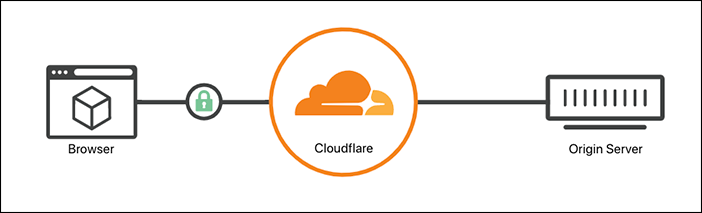
\includegraphics[width=0.8\linewidth]{cloudflare/flexible.png}
    \caption{Cloudflare con configurazione Flexible SSL}%
    \label{fig:flexiblessl}
\end{figure}

L'alternativa alle \emph{Flexible SSL} sono le \emph{Full SSL} (Figura~\ref{fig:fullssl}), queste aggiungono un secondo certificato tra Cloudflare \`e il sito web origine, il certificato pu\`o essere generato da Cloudflare gratuitamente, da Cerfication Authority oppure pu\`o essere generato localmente dall'azienda stessa. % Bib: https://support.cloudflare.com/hc/en-us/articles/200170416-End-to-end-HTTPS-with-Cloudflare-Part-3-SSL-options

\begin{figure}[htpb]
    \centering
    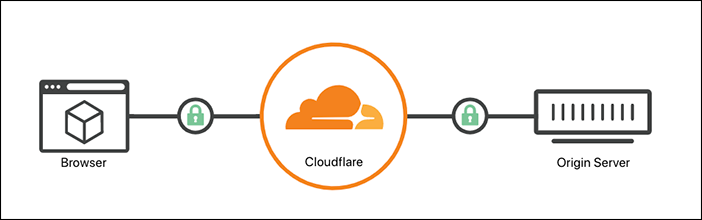
\includegraphics[width=0.8\linewidth]{cloudflare/full.png}
    \caption{Cloudflare con configurazione Full SSL}%
    \label{fig:fullssl}
\end{figure}

Il servizio per la prenotazione di spiaggie richiede l'utilizzo di Full SSL, tuttavia \`e richiesta completa fiducia verso Cloudflare: per permettere di individuare e filtrare i pacchetti malevoli, il traffico tra i visitatori e il server viene decifrato da Cloudflare e poi cryptato nuovamente con il secondo certificato. Cloudflare agisce come una VPN ad accesso remoto, il traffico viene cifrato tra il proxy e le sue fonti ma \textbf{il proxy ha accesso completo alle informazioni e pu\`o impersonare ogni utente}. Cloudflare \`e considerato affidabile dalle pi\`u grandi multinazionali del mondo ma \`e comunque necessario far presente di questa vulnerabilit\`a all'azienda. 